\documentclass[12pt]{article}
\usepackage[utf8]{inputenc}
\usepackage[a4paper, total={7in, 11in}]{geometry}
\usepackage{array}
 \usepackage{amsmath,amssymb}
 \usepackage{amsthm}
 \usepackage{bm}
 \usepackage{latexsym}
 \usepackage{CJK}
 \usepackage{multirow}
 \usepackage{caption}
 \usepackage{graphicx,color}
 \usepackage{amssymb,amsfonts}
 \usepackage{hyperref}
 \usepackage[english]{babel}
 \usepackage{times}
 \usepackage[T1]{fontenc}
 \usepackage{enumerate}
\usepackage{geometry}
\usepackage{float}
\usepackage{appendix}
\usepackage{booktabs}
\usepackage{endnotes}
\usepackage{mathtools}
\usepackage{amscd}
\usepackage{bbm}
\usepackage{multirow}
\usepackage{booktabs}
\usepackage{bm}
\renewcommand{\arraystretch}{1.1}
\renewcommand{\vec}{\bm}
%\usepackage{setspace}
\geometry{margin=1in}
\usepackage{graphicx}
\usepackage{amsmath}
\DeclareMathOperator{\sign}{sign}
%\usepackage{natbib}
\usepackage[numbers,sort&compress]{natbib}
\bibliographystyle{unsrt}
%\bibliographystyle{myapalike}
%\bibliographystyle{chicago}
\usepackage[scaled]{beramono}
\usepackage[T1]{fontenc}
%\usepackage{tgtermes}
%\usepackage{tgpagella}

\usepackage{amsmath,amsfonts,amssymb}
\usepackage{mathtools}
%\setcitestyle{aysep={}}
%\addtolength{\oddsidemargin}{-.5in}%
%\addtolength{\evensidemargin}{-.5in}%
%\addtolength{\textwidth}{1in}%
%\addtolength{\textheight}{1.3in}%
%\addtolength{\topmargin}{-.8in}%
%\linespread{1.6}
%\setlength{\parindent}{2em}
\usepackage{url}
\usepackage{hyperref}
\usepackage{setspace}
\usepackage{bbm}
\usepackage{fixltx2e}
\usepackage{graphicx}				
\usepackage{amsmath}
\usepackage{float}
\usepackage{subfig}

\title{Active Clustering with Unknown Evaluation Metric}
\author{Illinois Statistics Office}
\date{}

\begin{document}
\large
\maketitle

\section{Problem Formulation}
Given $N$ samples $X_i\in \mathbb{R}^m,~i=1,\cdots,N$ and a feature map $f: \mathbb{R}^m\rightarrow \mathbb{R}^p$ which maps $X_i$ to a $p$-dimensionl feature space. For the clustering task, we hod as a function $g$ to map the features to $K$ clusters: $g:\mathbb{R}^p\rightarrow \mathbb{R}, f(X)\longmapsto k,k=1,\cdots, K$. Additionally, we define a evaluation function $f$ to estimate the performance of the clustering method. Usually for clustering, this metric can be adjusted rand index \cite{hubert_comparing_1985}, mutual information based scores \cite{Vinh:2009:mutual} and so on. In our case, however, this evaluation metric is unknown and relies on the feedback of the human (or the oracle). Denote the function space of $g$ as $\mathcal{G}$, then the problem can be described as
\begin{equation}\label{original_problem}
\max_{g\in\mathcal{G}} h(g\circ f(\mathbf{X})).
\end{equation}
However, since we cannot exhaust the choices of $g\in \mathcal{G}$, we usually constrains our solution on a parameterized space with parameter ${\vec{\theta}}\in \mathbb{R}^q$, so that the optimization can be done on a $q$-dimensional Euclidean space. Denote the corresponding function as $g_{\vec{\theta}}$, then the problem (\ref{original_problem}) can be approximated by
\begin{equation}\label{para_problem}
\max_{\vec{\theta}\in\mathbb{R}^q } h(g_{\vec{\theta}}\circ f(\mathbf{X}))
\end{equation}

\section{Framework and Discussion}
First of all, to optimize $\vec{\theta}$, we need to get a reasonable estimation of $h$, which relies on the human interaction. We call the procedure of selecting samples and asking human for feedback as a "query". For each query, a pair of parameters $\vec{\theta_1}$ and $\vec{\theta_2}$ are chosen and the corresponding clustering method $g_{\vec{\theta_1}}$ and $g_{\vec{\theta_2}}$ are applied. The human then chooses $D<N$ samples and determine which clustering method is better, i.e., to inference if
\begin{equation}
h(g_{\vec{\theta_1}}\circ f(\vec{X}))>h(g_{\vec{\theta_2}}\circ f(\vec{X}))
\end{equation}
based on the performance of the $D$ chosen examples. The human interaction will continue until the budget runs out or the human fails to distinguish the difference of the performance of $g_{\vec{\theta_1}}$ and $g_{\vec{\theta_2}}$.

\textbf{In an active learning framework, the key of solution to (\ref{para_problem}) is to design an consistent and efficient query strategy to maximize $h(g_{\vec{\theta}}\circ f(\mathbf{X}))$ with limited attempts of $\vec{\theta$}.}

\textbf{ A sub-problem is to explore a sampling method of $D$ samples so they will represent the behavior of the two clustering method reasonably well}. 

For the sub-problem, an intuitive way is to select the samples that on the boundaries of the clusters like \cite{grira_active_2005}. After applying the clustering method $g_{\vec{\theta_1}}$ and $\vec{\theta_2}$, we can get two boundary sets$B_1$ and $B_2$ according to the two clustering results respectively. Then we can select the $D$ samples from $B_1\cup B_2$. However, the boundary based sampling method may result in sampling bias \cite{dasgupta_hierarchical_2008}.

For the main problem, our setting is quite different from that in the conventional active learning context. To be specific, in active supervised learning, the evaluation metric $h$ is always known. And instead of comparing the behavior of $g_{\vec{\theta_1}}$ and $g_{\vec{\theta_2}}$ to get an estimation of $h$, the performance of the model can be computed and compared directly. The human interaction here is to label new samples, which are used to train optimal $\vec{\theta}$. And based on optimized $\vec{\theta}$, people choose which unlabeled sample to be presented to the oracle. The loop continues until the budget is exhausted. In a more complex case \cite{raghavan2006active}\cite{druck_active_2009}, the human interaction is not limited to labeling the samples but also the features extracted by $f$.

On the other hand, for active unsupervised learning task, the metric $h$ is unknown, but it is under some constraints and does not require human to determine. For example, \cite{grira_active_2005} add "must-link" and "cannot-link" to the loss function. This is equivalent to consider $\ell_{\vec{\theta}}=h\circ g_{\vec{\theta}}$ and optimize it as a whole.


\section{Literature review}
\begin{itemize}
\item \cite{hofmann_active_1998} propose a scheme to improve the efficiency of clustering by performing the clustering procedure on the selected sample data instead of whole dataset. The original data is the proximity data that are similarity values obtained by comparing pairs of entities. The selection of  data for clustering is based on the expected value of information which measures the gain in  classification accuracy by incorporating addition data. 

\item \cite{druck_active_2009} propose a framework of active supervise learning, whose goal is to learn the output's distribution conditioned on the input features. The full conditional distribution of output is modeled through conditional random field. During each iteration in training, the algorithm ask user to label a feature selected by some information entropy criterion to reduce the model uncertainty. Specifically, this is not feature selection since we are not determining which features will be part of the model but determining the features for which supervisory feedback will be most helpful to the model.

\begin{figure}[H]
	\centering
	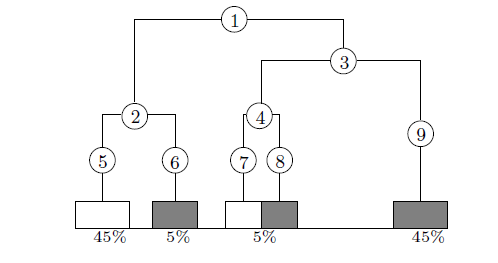
\includegraphics[width=0.7\linewidth]{hierarchical}
	\caption{Hierarchical clustering during active learning, from \cite{druck_active_2009}}
	\label{fig:hierarchical}
\end{figure}
\begin{figure}[H]
	\centering
	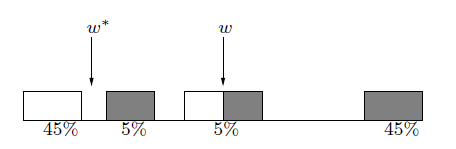
\includegraphics[width=0.7\linewidth]{hierarchical2}
	\caption{Shortcoming of the selection on the boundary and the consequent sampling bias}
	\label{fig:hierarchical2}
\end{figure}



\item \cite{dasgupta_hierarchical_2008} propose a hierarchical clustering based active learning algorithm. It divides the whole process into three steps: 1. hierarchical clustering 2. clustering adaptive sampling and labeling 3. supervised learning on the resulting fully labeled data. During step 2, it computes the weight based on the purity of the (labeled) subtrees and Wald's average linkage clustering. The advantage of the hierarchical tree based method is that it will avoid the "sampling bias" to some extent. The query part is asking the human to label/ classify the samples. (\textbf{The crieterion for pruning the hierarchical tree needs further review.(admissible set)})

\item \cite{grira_active_2005} combine the fuzzy clustering and active supervised learning. The boundary of the clusters are defined as the data points with the lowest probability that belongs to the cluster. The human is then asked to add constraints of "must-link" and "cannot-link" constraints of the "most valuable pairs" (MVP) based on the extended boundary to refine the clustering as shown in the figure below.

Notice: 1) The inputs in their experiment are extracted features (histograms) of dimension 100 instead of the original images. 2) They use Mahalanobis distance to compute the dissimilarity between the samples.
\begin{figure}[H]
	\centering
	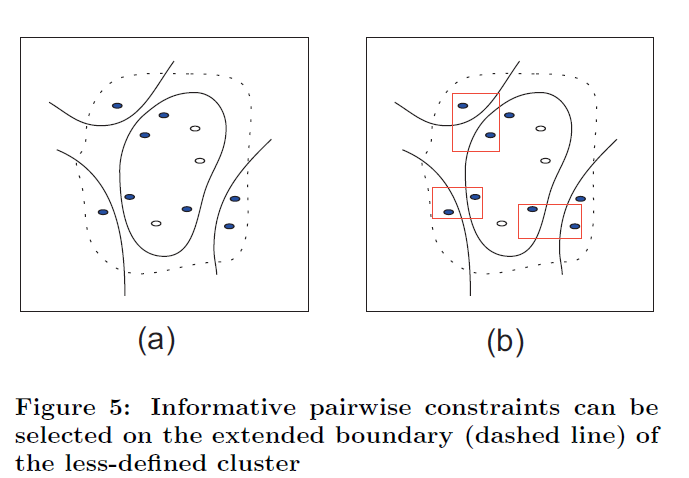
\includegraphics[width=0.7\linewidth]{mvp}
	\caption{Figure from \cite{grira_active_2005}}
	\label{fig:mvp}
\end{figure}

\item \cite{raghavan2006active} propose a framework of active learning to simultaneously using the user's feedback about the selected instances and features to improve the learning. During each iteration the model is retrained based on the instances and features selected from candidates, which are obtained based on information criterion. The training procedure stops when the budget of user supervision is reached. The main advantage is that the human-chosen features significantly accelerate learning compared to traditional active learning. 
\end{itemize}

\bibliography{activeclustering}
\end{document}